\documentclass{article}
\usepackage[spanish]{babel}   
\usepackage[numbers,sort&compress]{natbib}
\usepackage{float}
\usepackage{listings}
\usepackage{graphicx} 	% Nos permite importar imagenes 
\usepackage{subfigure}
\usepackage[left=3cm,right=3cm,top=3cm,bottom=3cm]{geometry}

%-------------------------- Por si se romple la URL --------------------------
\usepackage[hyphens]{url}
\usepackage[hidelinks]{hyperref}
\hypersetup{breaklinks=true}	
\urlstyle{same}
\usepackage{cite}
%-------------------------- Por si se romple la URL --------------------------

\title{Reporte Tarea 8}
\author{Victor Alejandro Oviedo Martínez}



\begin{document}
\maketitle
\hrule

\section{Introducción}\label{intro}
Para esta octava tarea \citep{DRA.P8} se ha estudiado el tema modelo de urnas, el cual es aplicado a la simulación de un sistema el cual tiene la función de coalescencia y fragmentación. En esencia, esta simulación tendrá una cantidad total de $n$ partículas, con las cuales formaran un tamaño inicial de $k$ cúmulos. Una vez teniendo los cúmulos se llevara acabo el proceso de fragmentación y coalescencia, en los cuales se dividirá los cúmulos para formar nuevos tamaños de los mismos, y luego volverán a unirse en el proceso de coalescencia. Este proceso podrá ser repetido un valor determinado.\\

Una vez determinado el valor de la variable $n$, generamos $k$, los cuales tendrán una distribución normal estándar para luego normalizarlos y convertirlos en enteros positivos que sumen a $n$. Para el proceso de fragmentación se utilizar la función sigmoidal centrada a la variable $c$ la cual es el promedio de los cúmulos iniciales, esto con el fin de fragmentar con mayor probabilidad los cúmulos de mayor tamaño y inversamente a los cúmulos de menor tamaño. En el caso de coalescencia, se utiliza la función exponencial con el fin de agrupar con mayor probabilidad los cúmulos de menor tamaño, y con menor probabilidad los cúmulos de mayor tamaño. Se tiene que en estos dos procesos es donde se utiliza el modelo urnas, ya que al momento de iniciar estos procesos es necesario saber cuántos cúmulos tenemos y la cantidad de partículas que contienen cada uno de ellos. Por lo tanto, se tendrán diferentes `urnas'' para cada diferente cúmulos que contengan la misma cantidad de partículas. De esta forma se podrá tener el control de los diferentes cúmulos y el movimiento de los mismos. De esta forma se lleva  acabo la simulación hasta un número determinado de iteraciones.\\




\section{Desarrollo}

Para esta séptima tarea se ha planteado el siguiente problema: Supongamos que cúmulos con $c$ o más partículas (haciendo referencia al tamaño crítico $c$) son suficientemente grandes para filtrar. Determina para diversas combinaciones de $k$, $n$ y el número de iteraciones $t$ cuál porcentaje de las partículas se logra filtrar si el filtrado se lleva a cabo después de $t$ iteraciones del proceso.\\

Para el desarrollo de esta tarea se ha utilizado el código ejemplo proporcionado por \citet{DRA.Code}, el cual tiene el propósito de: 
simular el proceso de coalescencia y fragmentación con valores específicos $n$ y $k$. Este código será tomado como base para entregar las características de esta tarea.\\

Para el desarrollo de esta tarea, se ha iniciado volviendo función el código proporcionado por \citet{DRA.Code}, y agregando el código necesario para devolver como resultado de esta función el porcentaje de las partículas filtradas. Este procedimiento se lleva acabo al final del procedimiento de iteraciones y se eliminan todos los valores superiores a la variable $c$.\\

\begin{lstlisting}[language=Python]
if paso == duracion-1:

            total = len(cumulos)
            filtrados = []
            nofiltrados = []
            for x in range(len(cumulos)):
                if cumulos[x] > c:
                    filtrados.append(cumulos[x])
                else:
                    nofiltrados.append(cumulos[x])

            PORfiltrados = ((len(filtrados)*100)/total)
            cumulos = nofiltrados

    return PORfiltrados 
\end{lstlisting}

Ya que el código regresa el valor requerido, se utilizara esta función para graficar los valores requeridos.

\begin{lstlisting}[language=Python]
k = [200, 400, 600, 800]
n = [20000,40000,60000,80000]
duracion = [25, 50, 75, 100]
rep = 10

digitos = floor(log(len(k), 10)) + 1

DIM_1 = []
DIM_2 = []
DIM_3 = []
for K in k:
    DIM_3 = []
    for N in n:
        print(N)
        DIM_2 = []
        for DURACION in duracion:
            DIM_1 = []
            for i in range(rep):
                res = fil(K, N, DURACION)
                DIM_1.append(res)
            DIM_2.append(DIM_1)
        DIM_3.append(DIM_2)
\end{lstlisting}


Cómo se pudo ver en el código anterior, este será el encargado de obtener los valores para los diferentes valores de \texttt{k}, \texttt{n}, y \texttt{duracion}. Por último, se grafícan los datos obtenidos. \\


\section{Conclusión}

Siguiendo las especificaciones de esta tarea se tiene como resultado la figura \ref{fig:cuadro.1}, \ref{fig:cuadro.2}, \ref{fig:cuadro.3}, y \ref{fig:cuadro.4}, en la cuales podremos encontrar para cada valor de \texttt{k}, \texttt{n}, y \texttt{duracion} su respuesta al porcentaje de cúmulos filtrados. Tomando en cuenta; \texttt{k = [200, 400, 600, 800]}, \texttt{n = [20000,40000,60000,80000]}, y \texttt{duracion = [25, 50, 75, 100]}, esto con 10 repeticiones por combinación.


\begin{figure}[H]
\begin{center}
	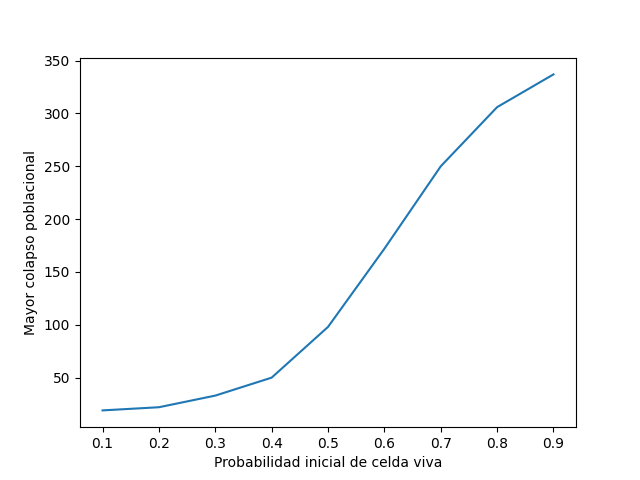
\includegraphics[height=3.5in]{/Users/victor/Desktop/Figure_1.png}
	\caption{ k = 200.}
	\label{fig:cuadro.1}
\end{center}
\end{figure}

\begin{figure}[H]
\begin{center}
	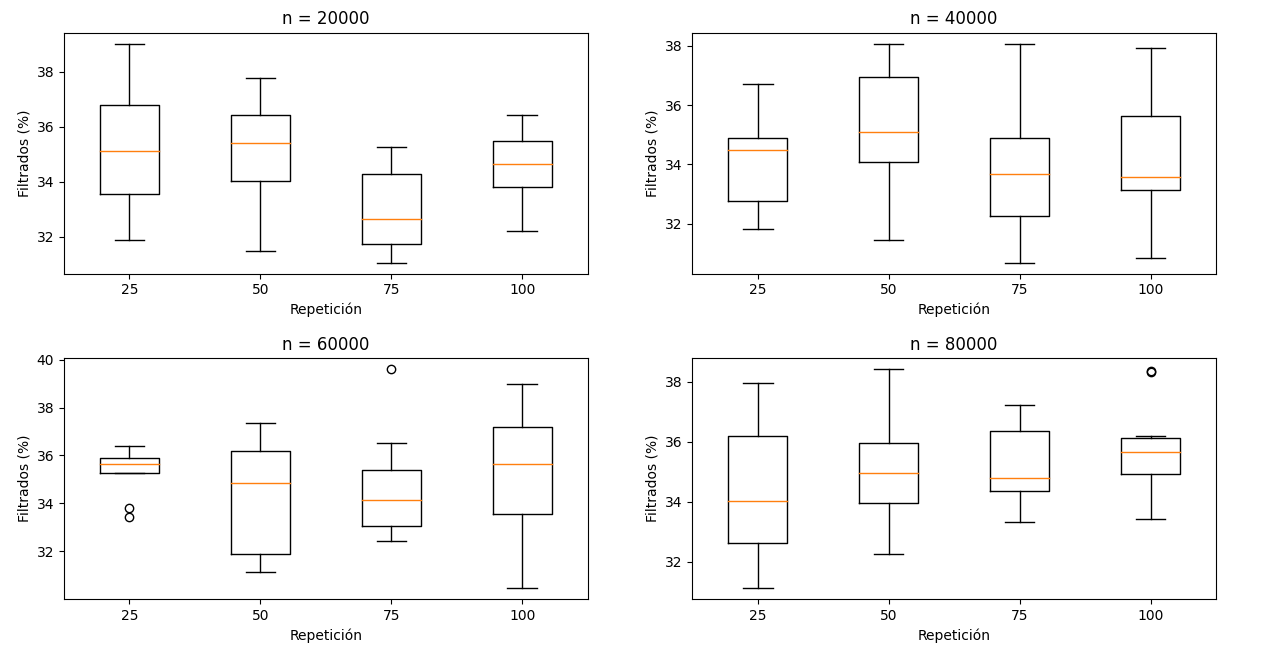
\includegraphics[height=3.5in]{/Users/victor/Desktop/Figure_2.png}
	\caption{ k = 400.}
	\label{fig:cuadro.2}
\end{center}
\end{figure}

\begin{figure}[H]
\begin{center}
	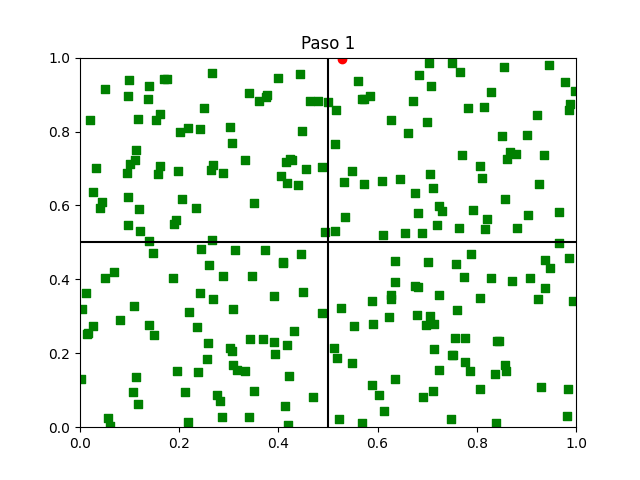
\includegraphics[height=3.5in]{/Users/victor/Desktop/Figure_3.png}
	\caption{ k = 600.}
	\label{fig:cuadro.3}
\end{center}
\end{figure}

\begin{figure}[H]
\begin{center}
	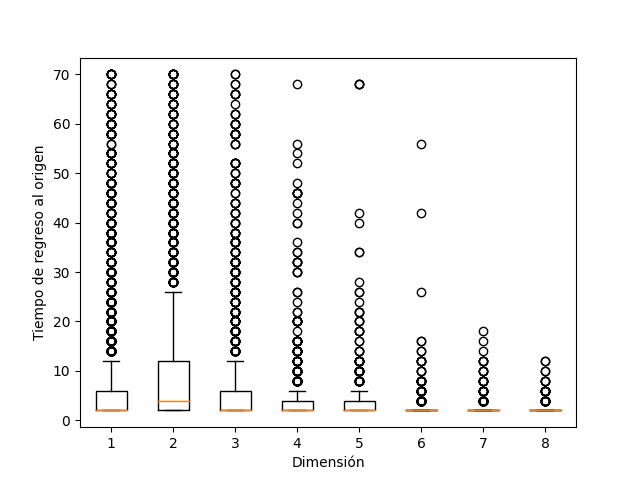
\includegraphics[height=3.5in]{/Users/victor/Desktop/Figure_4.png}
	\caption{ k = 800.}
	\label{fig:cuadro.4}
\end{center}
\end{figure}


%-------------------------- Por si se rompe la URL --------------------------
\Urlmuskip=0mu plus 1mu\relax
%-------------------------- Por si se rompe la URL --------------------------
\bibliography{ref.Tarea8.bib}
\bibliographystyle{plainnat}

\end{document}